\documentclass[12pt, a4paper, reqno]{amsart}
% ukazi za delo s slovenscino -- izberi kodiranje, ki ti ustreza
\usepackage[slovene]{babel}
\usepackage[T1]{fontenc}
\usepackage[utf8]{inputenc}
\usepackage{amsmath,amssymb,amsfonts,amsthm}
\usepackage{url}
%\usepackage[normalem]{ulem}
\usepackage[dvipsnames,usenames]{color}
\usepackage{graphicx}
\usepackage{tikz}
\usepackage{dsfont}
\usepackage{caption}
\usepackage{subcaption}
\usepackage{bm}
\usepackage{float}
\usepackage{xcolor}
\allowdisplaybreaks

% ne spreminjaj podatkov, ki vplivajo na obliko strani
\textwidth 15cm
\textheight 24cm
\oddsidemargin.5cm
\evensidemargin.5cm
\topmargin-5mm
\addtolength{\footskip}{10pt}
\pagestyle{plain}
\overfullrule=15pt % oznaci predlogo vrstico


% ukazi za matematicna okolja
\theoremstyle{definition} % tekst napisan pokoncno
\newtheorem{definicija}{Definicija}[section]
\newtheorem{zgled}[definicija]{Zgled}
\newtheorem{opomba}[definicija]{Opomba}

\renewcommand\endzgled{\hfill$\diamondsuit$}


\theoremstyle{plain} % tekst napisan posevno
\newtheorem{lema}[definicija]{Lema}
\newtheorem{izrek}[definicija]{Izrek}
\newtheorem{trditev}[definicija]{Trditev}
\newtheorem{posledica}[definicija]{Posledica}



% ukaz za slovarsko geslo
\newlength{\odstavek}
\setlength{\odstavek}{\parindent}
\newcommand{\geslo}[2]{\noindent\textbf{#1}\hspace*{3mm}\hangindent=\parindent\hangafter=1 #2}


% naslednje ukaze ustrezno popravi
\newcommand{\program}{Finančna matematika} % ime studijskega programa: Matematika/Finan"cna matematika
\newcommand{\imeavtorja}{Anej Rozman} % ime avtorja
\newcommand{\imementorja}{~doc.~dr. Martin Raič} % akademski naziv in ime mentorja
\newcommand{\naslovdela}{Sestavljeni Poissonov proces in njegova uporaba v financah} % naslov dela
\newcommand{\letnica}{2024} % letnica diplome

% Moji ukazi
\newcommand{\R}{\mathbb{R}}
\newcommand{\N}{\mathbb{N}}
\newcommand{\E}{\mathbb{E}}
\newcommand{\F}{\mathcal{F}}
\newcommand{\B}{\mathcal{B}}
\newcommand{\Prob}{\mathbb{P}}
\newcommand{\1}{\mathds{1}}
\newcommand{\Pois}[1]{\text{Pois}(#1)}
\newcommand{\Var}[1]{\text{Var}\left[#1\right]}





\begin{document}

\thispagestyle{empty}
\noindent{\large
UNIVERZA V LJUBLJANI\\[1mm]
FAKULTETA ZA MATEMATIKO IN FIZIKO\\[5mm]
\program\ -- 1.~stopnja}
\vfill

\begin{center}{\large
\imeavtorja\\[2mm]
{\bf \naslovdela}\\[10mm]
Delo diplomskega seminarja\\[1cm]
Mentor: \imementorja}
\end{center}
\vfill

\noindent{\large
Ljubljana, \letnica}
\pagebreak

\thispagestyle{empty}
\tableofcontents
\pagebreak

\thispagestyle{empty}
\begin{center}
{\bf \naslovdela}\\[3mm]
{\sc Povzetek}
\end{center}
% tekst povzetka v slovenscini

\vfill
\begin{center}
{\bf Compound Poisson process and its application in finance}\\[3mm] % angleski naslov
{\sc Abstract}
\end{center}
% tekst povzetka v anglescini
Prevod zgornjega povzetka v angle"s"cino.

\vfill\noindent
{\bf Math. Subj. Class. (2020):} 60G07 60G20 60G51 \\[1mm]
{\bf Klju"cne besede:} slu"cajni procesi, sestavljen Poissonov proces  \\[1mm]
{\bf Keywords:} stochastic processes, compound Poisson process
\pagebreak



% tu se zacne besedilo seminarja
\section{Uvod}

    Poissonov proces "steje "stevilo prihodov v danem "casovnem intervalu, kjer narava prihodov 
    sledi dolo"cenim omejitvam. Sestavljeni Poissonov proces je podoben 
    Poissonovemu, razen da je vsak prihod ute"zen z neko slu"cajno spremenljivko. Kot standarden
    primer si lahko predstavljamo stranke, ki gredo v trgovino. Njihovi prihodi sledijo Poissonovemu 
    procesu, znesek denarja, ki ga porabijo, pa sledi sestavljenemu Poissonovemu procesu.  
    Predpostavimo, da stranke, ki prihajajo v trgovino, sledijo Poissonovemu procesu z intenzivnostjo 
    $\lambda = 0.1$ in da je koli"cina denarja, ki ga porabijo, porazdeljena eksponentno s parametrom 
    $\alpha = 20$, torej na"sa trgovina ne omogo"ca vra"cil. Slika \ref{fig:slika1} prikazuje primer 
    zaslu"zka dneva poslovanja. Na osi $x$ je "cas, na osi $y$ pa kumulativna vsota vseh prihodov do nekega 
    trenutka v "casu.

    \begin{figure}[H]
        \centering
        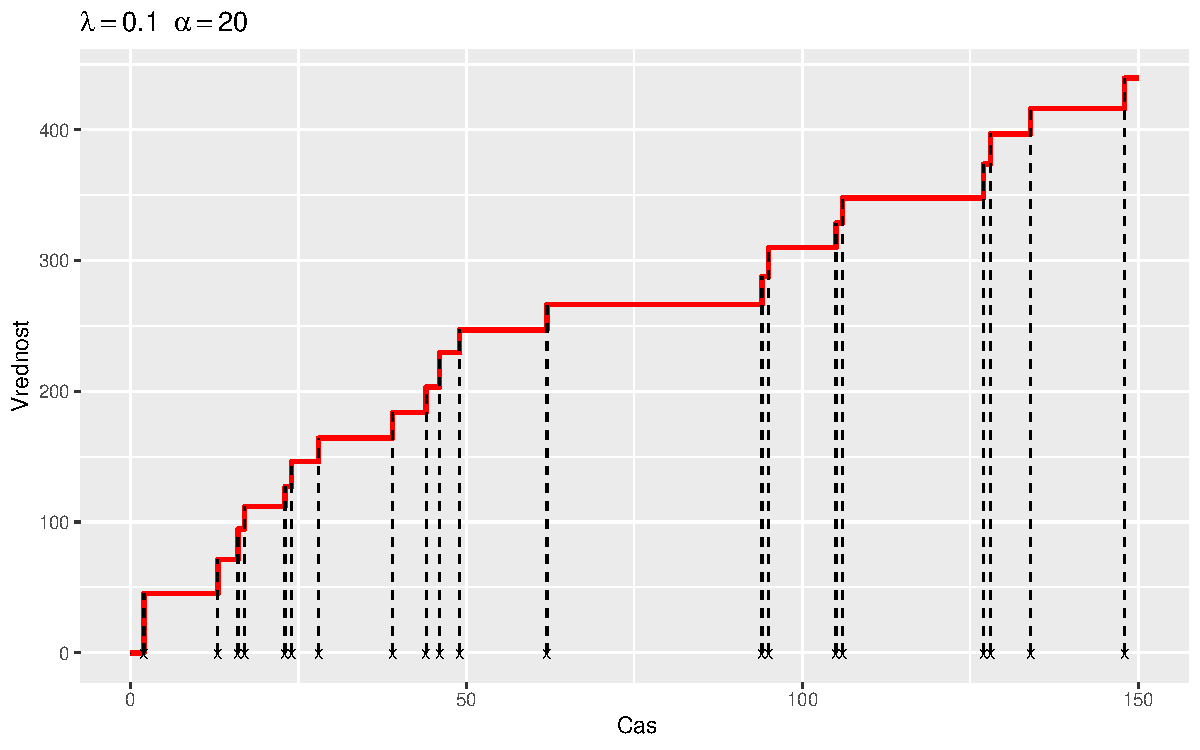
\includegraphics[width=\textwidth]{
            C:/Users/38651/OneDrive - Univerza v Ljubljani/Desktop/Diploma/Diplomski-seminar/GraphsAndPhotos/slika1.pdf
            }
        \caption{Primer trajektorije sestavljenega Poissonovega procesa}
        \label{fig:slika1}
    \end{figure}
    
    \noindent
\textcolor{red}{
    Vidimo, da je to zelo zanimiva ideja slu"cajnega
    procesa, ki ima veliko potencialnih uporab za modeliranje razli"cnih dogodkov. Na primer zahtevke 
    v zavarovalnici, "stevilo poivedb, ki jih prejema stre"znik, "spremembo v ceni nekega finan"cnega 
    instrumenta in mnoge druge. V delu bomo izpeljali osnovne lastnosti procesa ter se osredoto"cili 
    na njegovo uporabo v financah. Za za"cetek definirajmo osnovne pojme ter Sestavljen Poissonov proces.
}

    \begin{definicija}
        Naj bo $(\Omega, \mathcal{F}, \mathbb{P})$ verjetnostni prostor in naj bo $T\neq\emptyset$
        neprazna indeksna množica ter $(E, \Sigma)$ merljiv prostor. \textit{Slučajni proces}, 
        parametriziran s $T$, je družina slučajnih spremenljivk $X_t : \Omega \to E$,
         ki so $(\mathcal{F}, \Sigma)$-merljive za vsak $t \in T$.
        \label{def:slucProc}
    \end{definicija}

    \begin{opomba}
        Dr"zali se bomo konvencije, da $T$ predstavlja "cas, torej $T = [0, \infty)$ in da s.s.\
        zavzemajo vrednosti v realnih "stevili, torej $(E, \Sigma) = (\R, \B_{\R})$, kjer $\B_\R$ 
        predstavlja Borelovo $\sigma-$algebro na $\R$. Od tu dalje, "ce ni druga"ce navedeno, bomo 
        privzeli, da so s.s.\ definirane na nekem verjetnostnem prostoru 
        $(\Omega, \mathcal{F}, \mathbb{P})$ in zavzemajo vrednosti v $(\R, \B_{\R})$.
        \label{op:Konvencije}
    \end{opomba}


    \begin{definicija}
        Za fiksen $\omega \in \Omega$ je preslikava 
        $[0, \infty) \rightarrow \mathbb{R}; \ t \mapsto X_t(\omega)$ 
        \textit{trajektorija} oziroma \textit{realizacija} slučajnega procesa $(X_t)_{t\geq0}$.
        \label{def:realizac}
    \end{definicija}

\textcolor{red}{
    \begin{opomba}
        Na slu"cajni proces lahko gledamo tudi kot na predpis, ki nam iz vor"cnega prostora 
        $\Omega$ priredi slu"cajno funkcijo
        $(X_t(\omega))_{t\geq0}: [0, \infty) \rightarrow \mathbb{R}$.
        \label{op:slucFunkc}
    \end{opomba}
}
    \begin{definicija}
        Naj bo $(X_t)_{t\geq0}$ slu"cajni proces. Potem za $s < t$ definiramo
        \textit{prirastek procesa} $X_t - X_s$ na intervalu $[s, t]$. Proces $(X_t)_{t\geq0}$ ima 
        \textit{neodvisne prirastke}, če so za vsak nabor realnih "stevil
        $0 \leq t_1 < t_2 < \ldots < t_n < \infty$ prirastki
        $$
            X_{t_2} - X_{t_1}, \ X_{t_3} - X_{t_2}, \ \ldots, \ X_{t_n} - X_{t_{n-1}}
        $$
        med seboj neodvisni.
        \label{def:prirastek}
    \end{definicija}

    \begin{definicija}
        Naj bo $(X_t)_{t\geq0}$ slu"cajni proces. Potem pravimo, da ima proces
        \textit{stacionarne prirastke}, "ce za vsak $s < t$ in vsak $h > 0$ velja, 
        da ima $X_{t+h} - X_{s+h}$ enako porazdelitev kot $X_t - X_s$.
        \label{def:stacPrir}
    \end{definicija}

    \begin{definicija}
        Naj bo $\lambda > 0$. Slučajnemu procesu $(N_t)_{t\geq 0}$ definiranem na verjetnostnem 
        prostoru $(\Omega, \mathcal{F}, \mathbb{P})$ z vrednostmi v $\N_0$ pravimo 
        \textit{Poissonov proces} z intenzivnostjo $\lambda$, če zadošča naslednjim pogojem:
        \begin{enumerate}
            \item $N_0 = 0$ \ $\Prob$-skoraj gotovo.
            \item $(N_t)_{t\geq 0}$ ima neodvisne in stacionarne prirastke,
            \item Za $0 \leq s < t$ velja $ N_t - N_s \sim\Pois{\lambda(t - s)}$,
        \end{enumerate}
        \label{def:HPP}
    \end{definicija}
\textcolor{red}{
    \begin{opomba}
        Vidimo, da v definiciji ne zahtevamo, da so skoki procesa le +1. To sledi iz...
        \label{op:skoki}
    \end{opomba}
}
    \begin{definicija}
        Naj bo $(N_t)_{t\geq0}$ Poissonov proces z intenzivnostjo $\lambda$. 
        Naj bo $(X_i)_{i\geq1}$ zaporedje neodvisnih (med sabo in $N_t$) in enako 
        porazdeljenih slučajnih spremenljivk z vrednostmi v $\mathbb{R}$. Potem je 
        \textit{sestavljen Poissonov proces} $(S_t)_{t\geq0}$ definiran kot
        $$
            S_t = \sum_{i=1}^{N_t} X_i.
        $$
        \label{def:CPP}
    \end{definicija}

    \begin{opomba}
        Vidimo, da je Poissonov proces le poseben primer sestavljenega Poissonovega procesa, ko za
        $X_i$ vzamemo konstantno funkcijo $X_i = 1$ za vsak $i$. Bolj v splo"snem, "ce za $X_i$ 
        postavimo $X_i = \alpha$, potem velja $S_t = \alpha N_t$.
        \label{op:CPPHPPPovezava}
    \end{opomba}

    V nadaljevanju bomo Poissonovemu procesu rekli HPP (angl. Homogeneous Poisson Process) in ga
    ozna"cevali z $(N_t)_{t\geq0}$, sestavljenemu Poissonovemu procesu pa $CPP$ (angl. Compound Poisson 
    Process) in ga ozna"cevali s $(S_t)_{t\geq0}$. "Ce ni druga"ce navedeno, bo $\lambda$ ozna"cevala
    njuno intenzivnost.

\section{Lastnosti sestavljenega Poissonovega procesa}

    V tem poglavju si bomo ogledali osnovne lastnosti sestavljenega Poissonovega procesa. Pogledali
    si bomo... 
    \begin{trditev}
        $CPP$ ima neodvisne in stacionarne prirastke.
        \label{trd:neodvPrirCPP}
    \end{trditev}

    \begin{proof}
        Za nabor realnih "stevil $0 \leq t_1 < t_2 < \ldots < t_n < \infty$ lahko slu"cajne
        spremeljivke $S_{t_i} - S_{t_{i-1}}$ zapi"semo kot
        \begin{align*}
            S_{t_i} - S_{t_{i-1}} &= \sum_{j=N_{t_{i-1}}+1}^{N_{t_i}} X_j. 
        \end{align*}
        Neodvisnost prirastkov sledi po neodvisnosti $X_i$ od $X_j$ za $i\neq j$ in $N_t$. 
        Naj bo $h > 0$ in $s < t$. Potem velja
        \begin{align*}
            S_{t+h} - S_{s+h} &= \sum_{j=N_{s+h}+1}^{N_{t+h}} X_j \\
        \end{align*}
        Vsota ima $N_{t+h} - N_{s+h}$ členov. Ker za HPP velja 
        $N_{t+h} - N_{s+h} \sim N_t - N_s$, je 
        \begin{align*}
            \sum_{j=N_{s+h}+1}^{N_{t+h}} X_j = \sum_{j=N_{s}+1}^{N_{t}} X_j = S_t - S_s.
        \end{align*}
    \end{proof}

    Izra"cunajmo pri"cakovano vrednost in varianco $CPP$. Naj bo $(N_t)_{t\geq 0}$ HPP z 
    intenzivnostjo $\lambda$ in naj bo $\mu = \E\left[X_i\right]$ pri"cakovana vrednost 
    slu"cajnih spremenljivk $X_i$ za vsak $i$. Po formuli za popolno pri"cakovano vrednost velja 
    $\E\left[S_t\right] = \E\left[\E\left[S_t\mid N_t\right]\right]$. Torej

    \begin{align*}
        \E\left[S_t\right] &= \sum_{k=0}^{\infty} \E\left[S_t | N_t = k\right] \Prob\left(N_t = k\right)\\
                           &= \sum_{k=0}^{\infty} \E\left[\sum_{i=1}^{k} X_i\right] \Prob\left(N_t = k\right)\\
                           &= \sum_{k=0}^{\infty}k\E\left[X_i\right]\frac{(\lambda t)^k}{k!}e^{-\lambda t}\\
                           &= \mu\lambda te^{-\lambda t}\sum_{k=1}^{\infty}\frac{(\lambda t)^{k-1}}{(k-1)!}\\
                           &= \mu\lambda t.
    \end{align*}

    \noindent
    Za izra"cun variance potrebujemo dodatno predpostavko, da imajo slu"cajne spremenljivke $X_i$ 
    drugi moment. V tem primeru ozna"cimo $\Var{X_i} = \sigma^2$. Velja 
    $\Var{S_t} = \E\left[S_t^2\right] - \E\left[S_t\right]^2$, torej potrebujemo izra"cunati se 
    drugi moment. Ponovno uporabimo formulo za popolno pri"cakovano vrednost.
    \begin{align*}
        \E\left[S_t^2\right] 
                &= \sum_{k=0}^\infty\E\left[S_t^2\mid N_t = k\right]\Prob\left(N_t=k\right) \\
                &= \sum_{k=0}^\infty\E\left[\left(\sum_{i=1}^kX_i\right)^2\right]\Prob\left(N_t=k\right)\\
                &= \sum_{k=0}^\infty\E\left[\sum_{i=1}^kX_i^2 + \sum_{i\neq j}X_iX_j\right]\Prob\left(N_t=k\right)\\
                &= \sum_{k=0}^\infty\left(kE\left[X_i^2\right] 
                    +k(k-1)\E\left[X_i\right]\E\left[X_j\right]\right)\Prob\left(N_t=k\right)\\
    \end{align*}
    Prek formule $\Var{X_i} = \E\left[X_i^2\right] - \E\left[X_i\right]^2$ dobimo
    \begin{align*}
        \E\left[X_i^2\right] = \sigma^2 + \mu^2.
    \end{align*}
    Izraz $kE\left[X_i^2\right]+k(k-1)\E\left[X_i\right]\E\left[X_j\right]$ se tako poenostavi v 
    $k\sigma^2 + k^2\mu^2$, torej 
    \begin{align*}
        \E\left[S_t^2\right] 
                &= \sum_{k=0}^\infty\left(k\sigma^2 + k^2\mu^2\right)\Prob\left(N_t=k\right)\\
                &= \sigma^2\E\left[N_t\right] + \mu^2\E\left[N_t^2\right]\\
                &= \sigma^2\lambda t + \mu^2(\lambda t + \lambda^2t^2),
    \end{align*}
    kjer upo"stevamo, da $N_t \sim \Pois{\lambda t}$. Tako dobimo
    \begin{align*}
        \Var{S_t} 
                &= \sigma^2\lambda t + \mu^2(\lambda t + \lambda^2t^2) - (\mu\lambda t)^2 \\
                &= \sigma^2\lambda t + \mu^2\lambda t + \mu^2\lambda^2t^2 - \mu^2\lambda^2t^2\\
                &= \lambda t\left(\sigma^2 + \mu^2\right).
    \end{align*}

    \noindent
    Pojavi se vpra"sanje, kako pa je $S_t$ porazdeljena? Na to bomo odgovorili s pomo"cjo rodovnih
    funkcij. Naj bodo $X_1, X_2, \dots$ n.e.p. s.s.  z enako porazdelitvijo kot $X$.
    Izra"cunajmo momentno rodovno funckijo $CPP$. Ozna"cimo z $M_X(u)$ momentno rodovno funkcijo 
    s.s $X$ in z $M_{S_t}$ momentno rodovno funkcijo $CPP$.
    \begin{align*}
        M_{S_t}(u) 
                &= \E\left[\exp\left[uS_t\right]\right] =
                    \E\left[\exp\left[u\sum_{i = 1}^{N_t}X_i\right]\right]\\
                &= \Prob\left(N_t = 0\right) + \sum_{k=1}^{\infty}
                    \E\left[\exp\left[u\sum_{i = 1}^{N_t}X_i\mid N_t=k\right]\right]\Prob\left(N_t = k\right)\\ 
                &= \Prob\left(N_t = 0\right) + \sum_{k=1}^{\infty}
                    \E\left[\exp\left[u\sum_{i = 1}^kX_i\right]\right]\Prob\left(N_t = k\right)\\
                &= e^{-\lambda t} + \sum_{k=1}^{\infty}
                    \underbrace{\E\left[e^{uX}\right]^n}_{M_X(u)^n}\frac{(\lambda t)^k}{k!}e^{-\lambda t}\\ 
                &= e^{-\lambda t} + e^{-\lambda t}\sum_{k=1}^\infty\frac{\left(M_X(u)\lambda t\right)^k}{k!}\\
                &= e^{\lambda t\left(M_X(u) - 1\right)}    
    \end{align*}

    Iz opombe \ref{op:CPPHPPPovezava}, sledi, da "ce za $X_i$ vzamemo konstantno funkcijo 
    $X_i = 1$, dobimo HPP. Tako vidimo, da je momentno rodovna funkcija HPP enaka 
    $M_{S_t}(u) = e^{\lambda t\left(e^u - 1\right)}$. Poleg tega takoj dobimo, da sta 
    karakteristi"cna in rodovna funkcija $CPP$ enaki

    \begin{equation*}
        \varphi_{S_t}(u) = e^{\lambda t\left(\varphi_X(u) - 1\right)} \qquad \text{in} \qquad 
        G_{S_t}(u) = e^{\lambda t\left(G_X(u) - 1\right)}.
    \end{equation*} 

    \noindent
    V nadaljevanju bomo uporabljali predvsem karakteristi"cno funkcijo $CPP$, saj je ta vedno definirana 
    za vsak $u\in\R$.

    \noindent
    Sedaj se posvetimo vpra"sanju, kako je porazdeljena $S_t$? Iz definicije HPP vemo, da je 
    $N_t$ za $t\geq0$ porazdeljena kot Poissonova slu"cajna spremenljivka z intenzivnostjo 
    $\lambda t$. Fiksiramo $t\geq0$ in ra"cunamo

    \begin{align*}
        F_{S_t}(x) = \Prob(S_t \leq x) 
        &= \sum_{k=0}^\infty \Prob(S_t \leq x \mid N_t = k)\Prob(N_t = k) \\
        & = \sum_{k=0}^\infty \Prob(\sum_{i=1}^k X_i \leq x)\frac{(\lambda t)^k}{k!}e^{-\lambda t} \\
        & = \sum_{k=0}^\infty F_X^{*k}(x)\frac{(\lambda t)^k}{k!}e^{-\lambda t} \\
    \end{align*}

    \noindent
    kjer je $F_X^{*k}(x)$ porazdelitev $k$-te konvolucije slu"cajne spremenljivke $X$. Razen za 
    posebne primere, je zgornji izraz za prakti"cne namene ne-izra"cunljiv. 
    Poka"zimo, da je $CPP$ v resnici porazdeljena, kot limita linearne kombinacije neodvisnih Poissonovih
    slu"cajnih spremenljivk. Naj bodo $Y_1, Y_2, \dots, Y_n$ neodvisne s.s. porazdeljene 
    $\Pois{\lambda_1}, \ \Pois{\lambda_2}, \dots \Pois{\lambda_n}$. Ozna"cimo s $\varphi_{Z_n}(u)$ 
    karakteristi"cno funkcijo slu"cajne spremenljivke $Z_n = a_1Y_1 + a_2Y_2 + \dots + a_nY_n$ za neke 
    $a_1, a_2, \dots, a_n \in \R$.
    Potem po neodvisnosti velja

    \begin{align*}
        \varphi_{Z_n}(u) 
                &= \prod_{j=1}^{n}\varphi_{Y_j}(a_ju)\\
                &= \prod_{j=1}^{n}e^{\lambda_j\left(e^{a_j i u} - 1\right)} \\
                &= e^{\sum_{j=1}^{n}\lambda_j\left(e^{a_j i u} - 1\right)}.
    \end{align*}

    \noindent
    "Ce sedaj po"sljemo $n \to \infty$, dobimo
    \begin{align}
        \varphi_{Z}(u) := \lim_{n\to\infty}\varphi_{Z_n}(u) = e^{\sum_{j=1}^{\infty}\lambda_j\left(e^{a_j i u} - 1\right)}.
        \label{eq:karFunkcVrste}
    \end{align}

    \noindent
    Kot smo izpeljali zgoraj je karakteristi"cna funkcija $CPP$ podana s predpisom

    \begin{align*}
        \varphi_{S_t}(u) = e^{\lambda t\left(\varphi_X(u) - 1\right)}, 
    \end{align*}

    \noindent
    kar lahko zapi"semo kot 

    \begin{align*}
        \varphi_{S_t}(u) = e^{\lambda t\int_{\R}\left(e^{i u z} - 1\right) \mu(dz)},
    \end{align*}

    \noindent
    kjer je $\mu := X*\Prob$ potisk mere naprej po s.s.\ $X$. Prav tako lahko \ref{eq:karFunkcVrste} zapi"semo
    kot 

    \begin{align*}
        \varphi_{Z}(u) = e^{\int_{\R}\left(e^{i u x} - 1\right)\nu(dx)},
    \end{align*}

    \noindent
    Za neko ustrezno mero $\nu$. Vidimo, da ko po"sljemo $n\to \infty$, za ustrezen izbor 
    $a_1, a_2, \dots$ in $\lambda_1, \lambda_2, \dots$ karakteristi"cna funkcija 
    vrste $Z_n$ konvergira h karakteristi"cni funkciji $S_t$. Torej po Lévijevem izreku o zveznosti 
    sledi, da je $S_t$ enako porazdeljena kot $Z = \sum_{i=1}^{\infty}\alpha_iY_i$.

    \begin{zgled}
        "Ce pogledamo konkreten primer, ko so $X_1, X_2, \dots$ neodvisne s.s. porazdeljene eksponentno 
        s parametrom $\alpha$, lahko eksplicitno izra"cunamo porazdelitev $S_t$. Za $t\geq 0$
        in $x \geq 0$ velja
        \begin{align*}
            F_{S_t}(x) = \Prob(S_t \leq x)
            &= \sum_{k=0}^\infty F_X^{*k}(x)\frac{(\lambda t)^k}{k!}e^{-\lambda t}\\
            &= \sum_{k=0}^\infty \frac{\alpha^kx^{k-1}e^{-\alpha x}}{(k-2)!}\frac{(\lambda t)^k}{k!}e^{-\lambda t}\\
        \end{align*}
    \end{zgled}




    \subsection{$CPP$ kot martingal}

        \begin{definicija}
            Slu"cajni proces $X_t$ prilagojen glede na filtracijo $(\F_t)_{t\geq0}$
            martingal, "ce velja 
            $$
                \E\left[X_t\mid\F_s\right] = X_s
            $$
            za vsak $0\leq s \leq t$.
            \label{def:martingal}
        \end{definicija}

        Poka"zimo, da v splo"snem $CPP$ ni martingal.

        \begin{trditev}
            Naj bo $(S_t)_{t\geq0}$ $CPP$ z intenzivnostjo $\lambda>0$ in naj bodo $X_i$ neodvisne
            in enako porazdeljene slu"cajne spremenljivke z $\E\left[X_i\right] = \mu$ za vsak $i$.
            Potem je $S_t$ martingal natanko tedaj, ko je $\mu = 0$.
            \label{trd:CPPnimartingal}
        \end{trditev}

        \begin{proof}
            Naj bo $0\leq s\leq t$. Potem velja
            \begin{align*}
                \E\left[S_t\mid\F_s\right] 
                        &= \E\left[S_t - S_s + S_s\mid \F_s\right] \\
                        &= \E\left[S_t - S_s\right] + \E\left[S_s\mid \F_s\right] \\
                        &= \mu\lambda(t-s) + S_s
            \end{align*}
           Enakost $\mu\lambda(t-s) + S_s = S_s$ velja $\iff$ $\mu\lambda(t-s) = 0 \iff \mu = 0$.
        \end{proof}

        \begin{opomba}
            Seveda, "ce velja $\mu \geq 0$, potem je $S_t$ submartingal, "ce pa $\mu \leq 0$, je
            $S_t$ supermartingal.
        \end{opomba}

        \begin{trditev}
            Naj bo $(S_t)_{t\geq0}$ CPP z intenzivnostjo $\lambda > 0$ in naj bodo $X_i$ neodvisne
            in enako porazdeljene slu"cajne spremenljivke z $\E\left[X_i\right] = \mu$ za vsak $i$,
            Potem je proces 
            $$
                S_t - \mu\lambda t
            $$
            martingal.
            \label{trd:CPPpostanemartingal}
        \end{trditev}

        \begin{proof}
            Naj bosta $0 \leq s < t$. Prirastek $S_t - S_s$ je neodvisen od $\F_s$ in ima 
            pri"cakovano vrednost $\mu\lambda(t-s)$. Torej 
            \begin{align*}
                \E\left[S_t - \mu\lambda t\mid\F_s\right] 
                        &= \E\left[S_t - S_s\right] + S_s - \mu\lambda t\\
                        &= \mu\lambda(t-s) + S_s - \mu\lambda t\\
                        &= S_s - \mu\lambda s.
            \end{align*}
        \end{proof}

        \subsection{"Cas prvega prehoda}
        Postavimo si vpra"sanje, kdaj bo $CPP$ prvi"c dosegel nek $a\in\R$. Obravnavajmo primer, ko je 
        $a>0$, saj je primer, ko je $a$ negativen simetri"cen. Naj bo $T_a = \inf\{t\geq0; S_t \geq a\}$ 
        "cas prvega prehoda $CPP$. V tem poglavju bomo izra"cunali porazdelitev $T_a$.
        "Ce pogledamo dogodek $\{T_a \leq t\}$.

\section{Cramér-Lundbergov model}
    V nadaljevanju se bomo usmerili v Cramér-Ludenbergov model. Ta osnovni model za zavarovalni"ska
    tveganja je v svoji disretaciji leta 1903 prvi predstavil Fillip Lundeberg in tako postavil temelje
    za teorijo zavarovalni"stva. Kasneje je model je v tridesetih letih prej"snjega stoletja dopolnil 
    Harald Cramér. Osredoto"cili se bomo na koncept verjetnosti propada in njeno izražanje ali približevanje,
    ki se obravnava kot orodje za ocenjevanje tveganosti zavarovalniškega posla.

    \begin{definicija}
        Naj bo $(S_t)_{t\geq0}$ $CPP$ z intenzivnostjo $\lambda > 0$ in naj bodo $X_i$ n.e.p. s.s.
        z enako porazdelitvijo kot $X$ in $\E\left[X\right] = \mu$ ter $\Var{X} = \sigma^2$. Potem 
        \textit{proces tveganja} v Cramér-Lundbergovem modelu definiramo kot
        \begin{align*}
            U_t = u + ct - S_t,
        \end{align*}
        kjer je $u \geq 0$ za"cetni kapital zavarovalnice in $c>0$ stopnja prihodkov iz premij. 
        \label{def:procesTveganja}
    \end{definicija}

    Propad bomo definirali kot dogodek, ko bo vrednost procesa tveganja postala negativna.

    \begin{definicija}
        Za $0<T\leq\infty$ je \textit{Verjetnost propada} v Cramér-Lundbergovem modelu definirana kot
        \begin{align*}
            \psi(u, T) = \Prob(U_t < 0 \text{ za nek } T \geq t > 0), 
        \end{align*}
        "ce gledamo proces na kon"cnem intervalu in kot
        \begin{align*}
            \psi(u) = \Prob(U_t < 0 \text{ za nek } t > 0),
        \end{align*}
        "ce gledamo proces na neskon"cnem intervalu. Ozna"cimo "se 
        \begin{align*}
            \tau(T)=\inf\{t\mid T\geq t\geq, U_t <0 0\}, 
        \end{align*}
        kot \textit{"cas propada}, kjer se dr"zimo konvencije, da je $\inf\emptyset = \infty$ in 
        pi"semo $\tau = \tau(\infty)$ za "cas propada na neskon"cnem intervalu.
        \label{def:verjetnostPropadaInCasiPropada}   
    \end{definicija}

    Seveda takoj lahko opazimo, da je $\E\left[U_t\right] = u + ct - \E\left[S_t\right] = u + ct - \mu\lambda t$.
    Kar nam da prvo intuicijo o stopnji prihodkov premij $c$.



















\section*{Slovar strokovnih izrazov}

%\geslo{}{}
%
%\geslo{}{}
%


% seznam uporabljene literature
\begin{thebibliography}{99}

\bibitem{1}S.E. Shreve, Stochastic Calculus for Finance II: Continuous-Time Models, Springer, (2004).
\bibitem{2}S.M. Ross, Stochatic Processes: Second Edition, Wiley, (1996).
\end{thebibliography}

\end{document}